\documentclass[12pt, oneside, titlepage]{article}   	% use "amsart" instead of "article" for AMSLaTeX format

\usepackage{graphicx}
\graphicspath{ {\string} }
\usepackage{subcaption}

%%%%%%%%%%%%%%%%%%%%%%%%%%%%%%%%%%%%%%%%%%%%%%%%%%%%
% set up packages
%%%%%%%%%%%%%%%%%%%%%%%%%%%%%%%%%%%%%%%%%%%%%%%%%%%%
\usepackage{geometry}                
\usepackage{textcomp}                
\usepackage{amsmath}                
\usepackage{graphicx}                
\usepackage{amssymb}                
\usepackage{fancyhdr}                
\usepackage{subcaption}                
\usepackage{bm}                
\usepackage{tabularx}                

\usepackage{lineno}
% package for comments
\usepackage{soul}

\usepackage[breaklinks=true]{hyperref}

\usepackage[superscript,noadjust]{cite} % puts dash in citations to abbreviate
\usepackage [autostyle, english = american]{csquotes} % sets US-style quotes

\usepackage{etoolbox} % block quotes

\usepackage{float}
\usepackage{color}

\usepackage{pgf}
\usepackage{tikz}
\usepackage{eqnarray}

\usepackage{listings} % code blocks
\usepackage{setspace}

\usepackage{lscape}

% tikz background
\usetikzlibrary{backgrounds, fit}


\usepackage{natbib}
%\bibliographystyle{abbrvnat}
\setcitestyle{authoryear,open={(},close={)}}

%%%%%%%%%%%%%%%%%%%%%%%%%%%%%%%%%%%%%%%%%%%%%%%%%%%%
% call packages
%%%%%%%%%%%%%%%%%%%%%%%%%%%%%%%%%%%%%%%%%%%%%%%%%%%%	
\geometry{letterpaper, marginparwidth=60pt} % sets up geometry              		
\linenumbers % adds line numbers 
\MakeOuterQuote{"} % sets quote style
\doublespacing % setspace

%%%%%%%%%%%%%%%%%%%%%%%%%%%%%%%%%%%%%%%%%%%%%%%%%%%%
% patches with etoolbox 
%%%%%%%%%%%%%%%%%%%%%%%%%%%%%%%%%%%%%%%%%%%%%%%%%%%%	
% block quotes
\AtBeginEnvironment{quote}{\small}

% linenumbers
\makeatletter
\patchcmd{\@startsection}{\@ifstar}{\nolinenumbers\@ifstar}{}{}
\patchcmd{\@xsect}{\ignorespaces}{\linenumbers\ignorespaces}{}{}
\makeatother

%%%%%%%%%%%%%%%%%%%%%%%%%%%%%%%%%%%%%%%%%%%%%%%%%%%%
% tikzlibrary modifications
%%%%%%%%%%%%%%%%%%%%%%%%%%%%%%%%%%%%%%%%%%%%%%%%%%%%	
\usetikzlibrary{fit}
\usetikzlibrary{positioning}
\usetikzlibrary{arrows}
\usetikzlibrary{automata}

%%%%%%%%%%%%%%%%%%%%%%%%%%%%%%%%%%%%%%%%%%%%%%%%%%%%
% page formatting; exact 1 in margins
%%%%%%%%%%%%%%%%%%%%%%%%%%%%%%%%%%%%%%%%%%%%%%%%%%%%
\pagestyle{plain}                                                     

\setlength{\textwidth}{6.5in}    
\setlength{\oddsidemargin}{0in}
\setlength{\evensidemargin}{0in}
\setlength{\textheight}{8.5in}
\setlength{\topmargin}{0in}
\setlength{\headheight}{0in}
\setlength{\headsep}{0in}
\setlength{\footskip}{.5in}

%%%%%%%%%%%%%%%%%%%%%%%%%%%%%%%%%%%%%%%%%%%%%%%%%%%%
% defining code blocks using listings package
%%%%%%%%%%%%%%%%%%%%%%%%%%%%%%%%%%%%%%%%%%%%%%%%%%%%

\definecolor{dkgreen}{rgb}{0,0.6,0}
\definecolor{gray}{rgb}{0.5,0.5,0.5}
\definecolor{mauve}{rgb}{0.58,0,0.82}

\lstset{frame=tb,
  language=R,
  aboveskip=3mm,
  belowskip=3mm,
  showstringspaces=false,
  columns=flexible,
  basicstyle={\small\ttfamily},
  numbers=none,
  numberstyle=\tiny\color{gray},
 % keywordstyle=\color{blue},
  commentstyle=\color{dkgreen},
  stringstyle=\color{mauve},
  breaklines=true,
  breakatwhitespace=true,
  tabsize=3,
  otherkeywords={0,1,2,3,4,5,6,7,8,9},
  deletekeywords={data,frame,length,as,character,dunif,ps},
}

%%%%%%%%%%%%%%%%%%%%%%%%%%%%%%%%%%%%%%%%%%%%%%%%%%%%
%%%%%%%%%%%%%%%%%%%%%%%%%%%%%%%%%%%%%%%%%%%%%%%%%%%%
% begin document
%%%%%%%%%%%%%%%%%%%%%%%%%%%%%%%%%%%%%%%%%%%%%%%%%%%%
%%%%%%%%%%%%%%%%%%%%%%%%%%%%%%%%%%%%%%%%%%%%%%%%%%%%

\begin{document}

Last updated: \today

I evaluated convergence of the optimization routine using the following approach. The value function for optimization is 
%
\begin{align}
\mathrm{value} = \mathrm{objective} - \mathrm{weight_p} \times \mathrm{penalty} - \lambda \sum (\mathrm{wiggly}^2)
\end{align}

This is the objective in the optimal control problem, minus the penalty calculated during optimization (times a penalty weight), minus a penalty for the tortuosity of the solution (how wiggly the curve is). We chose to start with a large weight for the optimization penalty ($\mathrm{weight_p}=10$) and large weight for the tortuosity penalty ($\lambda=1$). We then ran the following routine: 

\begin{itemize}
\item Use the Runge-Kutta-4 method (rk4) for ODEs and Nelder-Mead for optimization (max $5000$ iterations).
\item Reset the controls to lie within their constraints.
\item Use the implicit Adams method (impAdams\_d, or impAdams) for ODEs and BFGS for optimization (max $1000$ iterations).
\item \hl{Reset the controls to lie within their constraints.}
\item Enter an optimization loop. Within the loop:
\subitem Use the implicit Adams method (impAdams or impAdamsd) for ODEs and Nelder-Mead for optimization (max $2500$ iterations).
\subitem Reset the controls to lie within their constraints.
\subitem Use the implicit Adams method (impAdams or impAdamsd) for ODEs and BFGS for optimization (max $1000$ iterations).
\subitem Reduce the weight for lambda by half.
\subitem \hl{GS: Is there a reason we might want to reduce the weight for constraint violation by half as well?}
\end{itemize}

I initially tested for how to optimize on the problem for unbranched, determinate plants with a objective function of $\log(F)$, a Uniform(0,5) season length distribution, initial states of [1,.1,0,.0001] and meristem constraints of [.75,1]. I experimented with modifying the following variables: number of iterations of the optimization routine, number of Nelder-Mead iterations, progression of penalty on tortuosity ($\lambda$ values).

Try removing the constraints from the for loop (SPE). I did this because the value of the optimization routine decreased over time but had some bumps where it decreased then increased again. Steve suggested this might be because of the constraints in the for-loop. I did that but it seemed to really change the solution. So I tried to break the problem apart a bit more. 

At each iteration, I kept the (1) value function from optimization, (2) the objective function, (3) the penalty for violating constraints, and (4) the difference of (-1 - (2 - 3)) which I think should approximate the penalty for tortuosity. Dips in the value function were associated with jumps in the objective function but also with the penalty for violating constraints. So I'm going to try running this again, for longer, without any constraints and see what that looks like. 

Graph the quadratic vs. 1.25 loss function. One thought is that maybe the penalty weight of 10 is too high because the loss function shape is different. Instead, I started at a penalty weight of 1, then increased to 10 after 10 iterations. This seemed to be the equivalent of going from 10 to 100 for a quadratic loss function, but with different behavior for very small values.

\begin{lstlisting}
plot(seq(-1,1,by=0.01),seq(-1,1,by=0.01)^2,type='l',xlim=c(-.25,.25))
lines(seq(-1,1,by=0.01),10*seq(-1,1,by=0.01)^2,lty='dashed')
lines(seq(-1,1,by=0.01),100*seq(-1,1,by=0.01)^2,lty='dotted')
lines(seq(-1,1,by=0.01),abs(seq(-1,1,by=0.01))^1.25,col='red')
lines(seq(-1,1,by=0.01),10*abs(seq(-1,1,by=0.01))^1.25,col='red',lty='dashed')
lines(seq(-1,1,by=0.01),100*abs(seq(-1,1,by=0.01))^1.25,col='red',lty='dotted')
\end{lstlisting}

It seems like putting both the penalty weight equal to 1 and the lambda equal to 1 initially led to better properties for the solution (in run 1). In round 2 of optimization I then increased the penalty weight to 10. I'm not sure if it ran for longer (?) but the solution seemed smoother, which may be because the solution worked to optimize the objective function first with a smaller penalty for constraint violations and only later imposed a stronger cost for constraint violations. One thing is that the value function decreased through the first round of optimization (with a set penalty weight) and then went up after I increased the penalty. Not sure what to make of that?


\singlespace

\begin{center}
\captionof{table}{ Summary of convergence tests. } \label{tab:title1} 
 \begin{tabularx}{\linewidth}{l l l l} 
 \hline
 \hline
  \multicolumn{1}{ c }{ Optimization iterations } & 
 \multicolumn{1}{ c }{ Nelder-Mead iterations } & 
\multicolumn{1}{ c }{ BFGS iterations } & 
\multicolumn{1}{ c }{ $\lambda$  }  \\
 \hline
 %%%% VIABILITY TRIALS
% \multicolumn{2}{ l }{ \sc{Viability trials }} \\

20 &  2500 & 1000 & 1, halve for (2-20) \\
20 &  2500 & 1000 & 1, halve for (1-10), 0 for (11-20) \\
20 &  5000 & 1000 & 1, halve for (1-10), 0 for (11-20) \\
30 &  2500 & 1000 & 1, halve for (2-30) \\
50 &  2500 & 1000 & 1, halve for (2-50) \\

  \hline
\end{tabularx}
\end{center}

\doublespace

\clearpage
\newpage

 \begin{figure}[h]
   \centering
       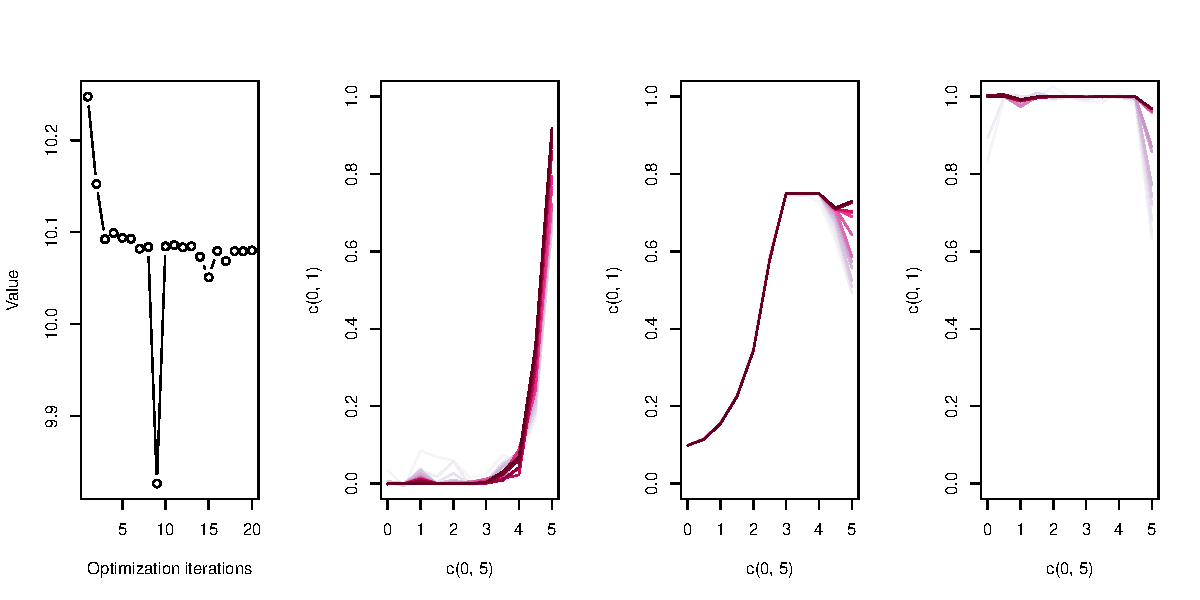
\includegraphics[width=1\textwidth]{../unbranched-determinate-convergence-2500-1000-2.pdf}  
    \caption{ Optimization: 20 iterations, Nelder-Mead: 2500 iterations, BFGS: 1000 iterations, start lambda at 1, halve for 2-20  }
 \label{fig:test}
\end{figure}

 \begin{figure}[h]
   \centering
       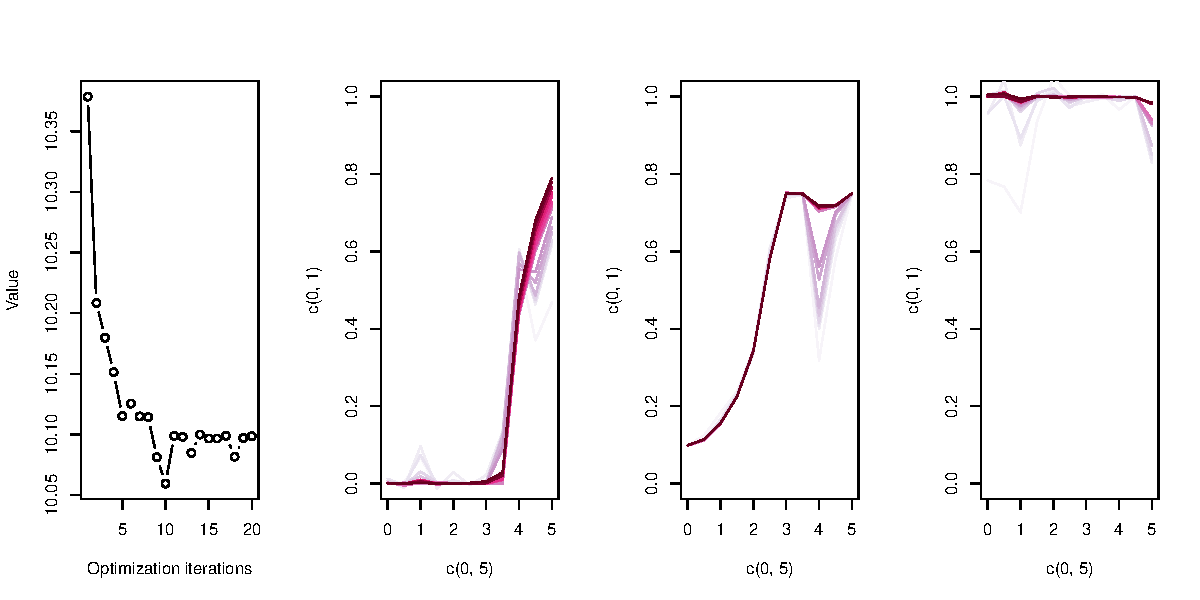
\includegraphics[width=1\textwidth]{../unbranched-determinate-convergence-2500-1000-lambda0-2.pdf}  
    \caption{ Optimization: 20 iterations, Nelder-Mead: 2500 iterations, BFGS: 1000 iterations, start lambda at 1, halve for (1-10), 0 for (11-20)  }
 \label{fig:test}
\end{figure}

 \begin{figure}[h]
   \centering
       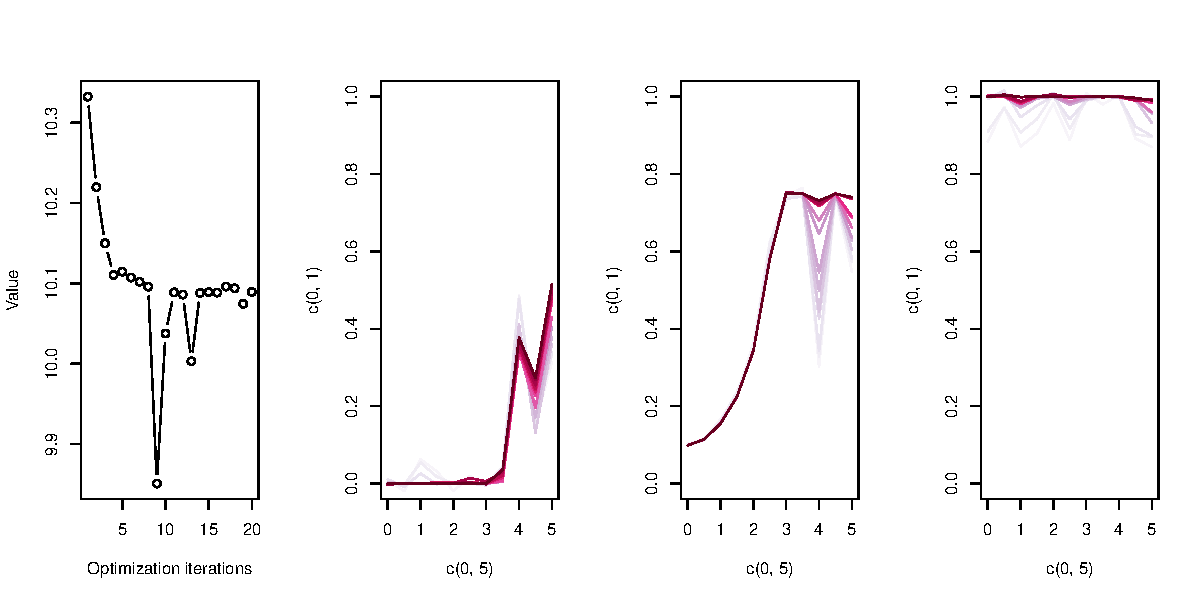
\includegraphics[width=1\textwidth]{../unbranched-determinate-convergence-5000-1000-lambda0-2.pdf}  
    \caption{ Optimization: 20 iterations, Nelder-Mead: 5000 iterations, BFGS: 1000 iterations, start lambda at 1, halve for (1-10), 0 for (11-20) }
 \label{fig:test}
\end{figure}

 \begin{figure}[h]
   \centering
       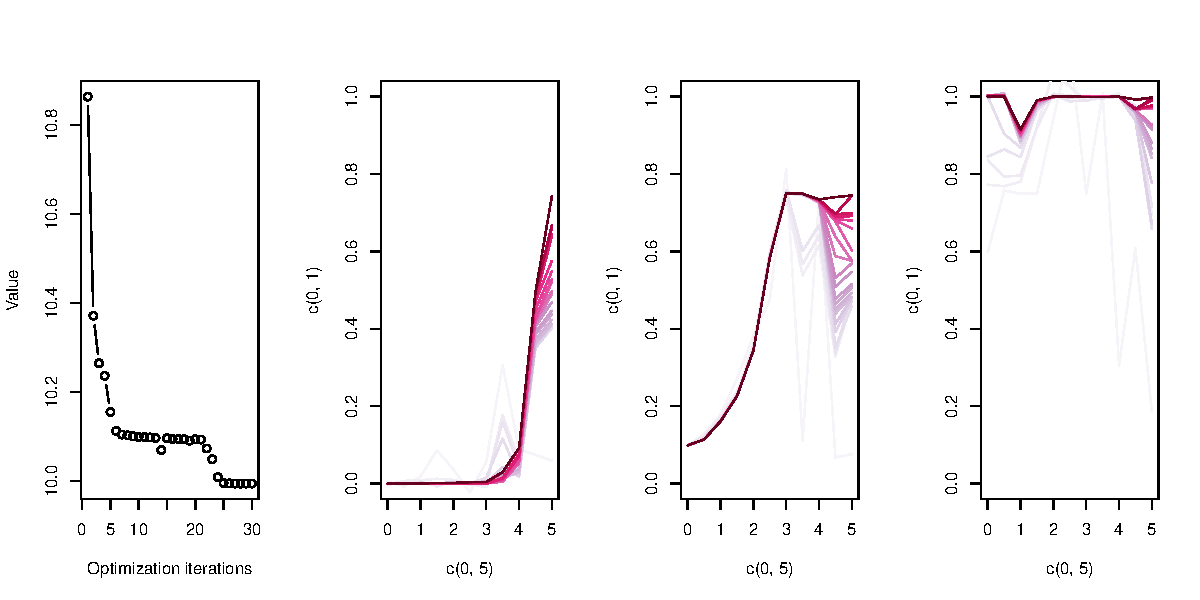
\includegraphics[width=1\textwidth]{../unbranched-determinate-convergence2500-1000-30iter-2.pdf}  
    \caption{ Optimization: 30 iterations, Nelder-Mead: 5000 iterations, BFGS: 1000 iterations, start lambda at 1, halve for (1-10), 0 for (11-30) }
 \label{fig:test}
\end{figure}

 \begin{figure}[h]
   \centering
       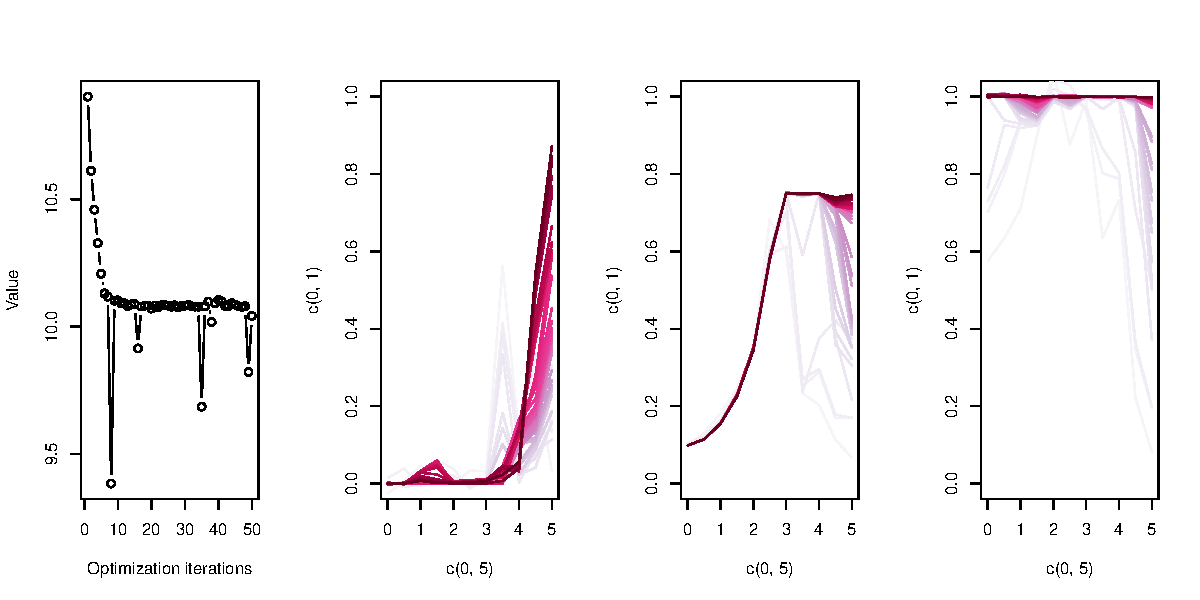
\includegraphics[width=1\textwidth]{../unbranched-determinate-convergence2500-1000-50iter-2.pdf}  
    \caption{ Optimization: 50 iterations, Nelder-Mead: 5000 iterations, BFGS: 1000 iterations, start lambda at 1, halve for (1-10), 0 for (11-50) }
 \label{fig:test}
\end{figure}

\end{document}
